\documentclass{beamer}

\usepackage{amsfonts,amsmath,comment,graphicx}

\title{Spectral Rigid Body Dynamics}
\author{Mikola Lysenko}

\begin{document}

\newcommand{\R}{\mathbb{R}}
\newcommand{\ind}[1]{{\bf 1}_{#1}}
\newcommand{\inner}[2]{\left \langle #1 , #2 \right \rangle}
%\newcommand{\exp}{\mathop{\text{exp}}}

\maketitle

\begin{frame}
	\frametitle{Overview}
		\tableofcontents
\end{frame}

\section{Rigid Body Dynamics}
\begin{frame}
\frametitle{Rigid Body Dynamics}
An approximate model of low energy physics for stiff objects

\pause
\vskip15pt
Pros:
\begin{itemize}
	\item{+} Pretty accurate at human energy scales
	\item{+} Good for stiff materials (ie metals, plastics etc.)
	\item{+} Easy kinematic constraints (useful for mechanisms)
	\item{+} Standard animation tool (videogames!)
\end{itemize}

\pause
\vskip15pt
Cons:
\begin{itemize}
	\item{-} Inaccurate at extremely large energies
	\item{-} Bad for materials with low elastic modulus
	\item{-} Not always solvable! (See: Painleve's paradox)
\end{itemize}
\end{frame}

\begin{frame}
\frametitle{What is a Rigid Body?}
An idealized solid object with elastic modulus $= \infty$
\pause
\vskip5pt
We identify a body $B$ with a scalar field, $\varphi : \R^d \to \R^+$
\vskip5pt
\begin{center}
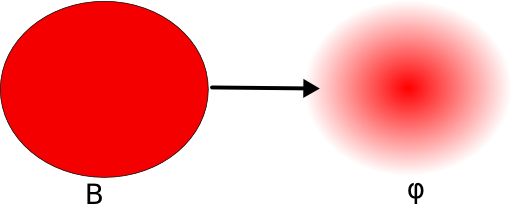
\includegraphics[height=1.1in]{figures/massfield.png}
\end{center}
\pause
\vskip5pt
$\varphi$ represents the mass distribution of $B$
\pause
\vskip5pt
$\varphi(x) = 0$ indicates $B$ does not occupy the space at $x$
\end{frame}

\begin{frame}
\frametitle{Configuration Space of a Rigid Body}
Transformations of rigid mass fields must preserve distance and handedness
\pause
\vskip5pt
In other words, must be a direct Euclidean isometry
\vskip5pt
Isomorphic to finite dimensional Lie group, $SE(d) \cong SO(d) \ltimes \R^d$
\vskip5pt
\pause
\begin{columns}
	\column{.5\textwidth}
		\begin{center}
		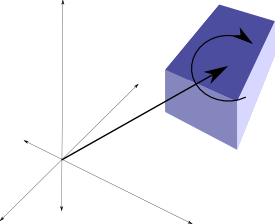
\includegraphics[height=1.4in]{figures/rigidbody.png}
		\end{center}
		
	\column{.5\textwidth}
		\begin{center}
		Can be parameterized by a translation $t$ and a rotation $R$
		
		\vskip15pt
		
		Matrix:
		$\left( \begin{array}{cc}
			R & t \\
			0 & 1 \\
		\end{array} \right)$
		
		\vskip15pt
		${d+1 \choose{2}}$ degrees of freedom
		
		\vskip15pt
		Tangent space: $\mathfrak{so}(d+1)$
		\end{center}
\end{columns}
\pause
\vskip10pt
\begin{center}
\bf{Motions of rigid objects $\cong$ curves $q(t) \subset SE(d)$}
\end{center}
\end{frame}


\section{Lagrangian Mechanics}
\begin{frame}
\frametitle{Lagrangian Mechanics}
Turns physics into an optimization problem.
\vskip5pt
\pause
Given a configuration curve $q$ at time $t$, define the \emph{Lagrangian}
\[ \mathcal{L}(q, \dot{q}, t) = T(\dot{q}) - U(q, t) \]
Where $T(\dot{q}) = \frac{1}{2} \dot{q}^T M \dot{q}$ is the kinetic energy and $U$ is a potential
\vskip15pt
\pause
{\bf Hamilton's Principle of Least Action}:
\begin{center}
	\emph{Physically plausible motions do minimal work}
\end{center}
\vskip10pt
\pause
In other words:
\[ \mathop{\text{argmin}}_{q : [t_0, t_1) \to SE(d)} \int \limits_{t_0}^{t_1} L(q, \dot{q}, t) dt \]
\end{frame}

\begin{frame}
\frametitle{Forward Kinematics}
Solve:
\[ \mathop{\text{argmin}}_{q : [t_0, t_1) \to SE(d)} \int \limits_{t_0}^{t_1} L(q, \dot{q}, t) dt \]
\pause
This is a 1st order variational problem, so use Euler-Lagrange:
\[ \frac{d}{dt} \left ( \frac{\partial L(q, \dot{q}, t)}{\partial \dot{q}} \right) = \frac{\partial L(q, \dot{q}, t)}{\partial q} \]
\pause
Unpack definitions and simplify:
\begin{eqnarray*}
\frac{d}{dt} \left( \frac{\partial \frac{1}{2} \dot{q}^T M \dot{q} }{\partial \dot{q}} \right) & = & \frac{\partial U(q, t)}{\partial q} \\
\pause
M \ddot{q} & = & \nabla U
\end{eqnarray*}
Newton's equations!
\end{frame}

\begin{frame}
\frametitle{Multiple Bodies}
Q: How to deal with multiple independent bodies?
\pause
\vskip5pt
A: Tensor sum
\vskip15pt
Let $B_i, B_j$ be independent rigid bodies with motions $q_i, q_j$
\vskip15pt
\begin{tabular}{ll}
Configuration space & $SE(d)^2 \cong SE(d) \oplus SE(d)$ \\
Motion & $q(t) \cong q_i(t) \oplus q_j(t)$ \\
Lagrangian & $L(q,\dot{q},t) = L(q_i, \dot{q}_i, t) + L(q_j, \dot{q}_j, t)$ \\
\end{tabular}
\pause
\vskip15pt
Scales to $n$ bodies, get Lagrangian in $SE(d)^n$
\end{frame}


\section{Standard Collisions}
\begin{frame}
\frametitle{Collisions}
Solids can't physically occupy the same space.
\vskip10pt
\begin{columns}
	\column{.5\textwidth}
		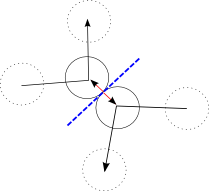
\includegraphics[height=2in]{figures/collision.png}
		\vskip5pt
		Need to keep them separated
		
	\pause
	\column{.5\textwidth}
	
	{\bf Standard method:}
	
	\begin{itemize}
	\item Time step to point of impact
	\pause
	\item Determine contact manifold
	\pause
	\item Apply penalty force/impulse to separate objects
	\pause
	\item Iterate until all collisions are resolved
	\end{itemize}
	\pause
	\vskip5pt
	+ Just like high school physics
	
\end{columns}
\end{frame}


\begin{frame}
\frametitle{Problems with typical collision methods}
Handling collisions this way is hard
\vskip5pt
\pause
\begin{itemize}
\item{-} Finding exact point/time of impact is expensive
\item{-} Contact manifolds can be difficult to classify
\item{-} Normal forces are ambiguous for curvy shapes
\item{-} Impulses are discontinuous; results in stiff system
\item{-} Penalty methods don't gaurantee separation
\item{-} Convergence properties not well understood
\item{-} Unclear how to handle sharp corners
\item{-} Discontinuity in simulation
\item{-} Complicated, ad-hoc
\end{itemize}
\pause
But can be made to work with enough hacking...
\end{frame}

\begin{frame}
\frametitle{There has got to be an easier way...}
\pause
Minimal requirement for physical plausibility
\vskip7pt
\begin{center}
\emph{At all times no two solids intersect}
\end{center}
\pause
\vskip15pt
Is this really all there is to it?

\end{frame}

\section{Constraint Based Collisions}
\begin{frame}
\frametitle{Constraint Based Impacts}
For any body $B_i$ with mass field $\varphi_i$, define the set:
\[ A_i = \kappa \iota \text{ supp } \varphi \]
\pause
So two solids, $A_i, A_j$, \emph{collide} at a configuration $q_i, q_j$ iff:
\[ \text{collide}(q_i A_i, q_j A_j) \Leftrightarrow \iota (q_i A_i \cap q_j A_j) \neq \emptyset \]
\pause
But,
\[ \iota ( q_i A_i \cap q_j A_j ) \neq \emptyset \Leftrightarrow \text{vol } q_i A_i \cap q_j A_j > 0 \]
\pause
Define
\[ C_{i,j}(q_i, q_j) \stackrel{def}{\equiv} \text{vol } q_i A_i \cap q_j A_j \]
And so we replace the impact forces with a system of differentiable holonomic inequality constraints:
\[ C_{i,j} \leq 0 \]
\end{frame}

\begin{frame}
\frametitle{Equations of motion revisited}
New problem:
\[ \text{minimize } \int \limits_{t_0}^{t_1} L(q, \dot{q}, t) dt \]
\[ \text{subject to } C_{i,j}(q_i, q_j) \leq 0 \:\:\: \forall t \in [t_0, t_1), i \neq j \]
\pause
Apply KKT conditions + Euler-Lagrange to get complementarity problem:
\[ \frac{d}{dt} \left( \frac{\partial T(\dot{q}_i)}{\partial \dot{q}_i} \right)
- \frac{\partial U(q, t)}{\partial q_i} + \alert<3>{\sum \limits_{j \neq i} \mu_{i,j} \frac{ \partial C_{i,j}(q_i, q_j)}{ \partial{q_i} }} = 0 \]
\[ \alert<3>{0 \leq \mu_{i,j} \perp -C_{i,j} \geq 0} \]
\pause
Exactly elastic collision response!
\vskip5pt
Slack variables are impulse forces
\end{frame}

\begin{frame}
\frametitle{Calculating $C_{i,j}$}
Need to compute:
\[ C_{i,j}(q_i, q_j) = \text{vol } q_i A_i \cap q_j A_j \]
\pause
Construct the \emph{indicator} on $A$
\[ \ind{A}(x) = \left \{ \begin{array}{cc}
1 & \text{if } x \in A \\
0 & \text{otherwise}
\end{array} \right. \]
\pause
Observe:
\begin{columns}
	\column{.5\textwidth}
		{\centering
		\[ \ind{A_i \cap A_j}(x) = \ind{A_i}(x) \ind{A_j}(x)  \]
		}
	
	\column{.5\textwidth}
		{\centering
		\[ \text{vol } A_i = \int \limits_{\R^d} \ind{A_i}(x) dx \]
		}
\end{columns}
\pause
So:
\[ C_{i,j}(q_i, q_j) = \int \limits_{\R^d} \ind{A_i}(q_i^{-1} x) \ind{A_j}(q_j^{-1} x) dx \]
\end{frame}

\begin{frame}
\frametitle{Calculating $C_{i,j}$ (cont.)}
\[ C_{i,j}(q_i, q_j) = \int \limits_{\R^d} \ind{A_i}(q_i^{-1} x) \ind{A_j}(q_j^{-1} x) dx \]
\pause
Push terms to one side:
\[ \int \limits_{\R^d} \ind{A_i}(x) \ind{A_j}(q_j^{-1} q_i x) dx \]
\pause
Substitute $q_j^{-1} q_i x \mapsto R(x - y)$ and let $\widetilde{\ind{A_j}}(x) = \ind{A_j}(-x)$:
\[ \int \limits_{\R^d} \ind{A_i}(x) \widetilde{\ind{A_j}}(R(y - x)) dx \]
\pause
So,
\[ C_{i,j}(q_i, q_j) = (\ind{A_i} \star (\widetilde{\ind{A_j}} \circ R))(y) \]
\end{frame}

\section{Fourier Methods}
\begin{frame}
\frametitle{Fourier Methods}
Convolution? \invisible<1>{Take a Fourier transform!}
\[ C_{i,j}(q_i, q_j) = (\ind{A_i} \star (\widetilde{\ind{A_j}} \circ R))(y)
\pause
= \mathcal{F}^{-1} \left ( \widehat{\ind{A_i}} \overline{\left(\widehat{\ind{A_j}} \circ R \right)} \right )(y) \]
\pause
What about gradients? (ie $\frac{\partial C_{i,j}(q_i, q_j)}{\partial q_i}$)
\pause
\vskip5pt
\vskip5pt
\begin{columns}
	\column{.5\textwidth}
		{\centering
		Fix parameters $q_i = (R_i, t_i)$, 
		\[q_i x = R_i x + t_i \]
		\[q_i^{-1} = (R_i^{-1}, -R_i^{-1} t_i) \]
		\[q_j q_i^{-1} x = R(x - y)\]
		}
	\column{.5\textwidth}
		\pause
		{\centering
		Solve for $R, y$,
		\[ R = R_j R_i^{-1} \]
		\[ y = R_i R_j^{-1} t_j - t_i \]
		}
\end{columns}
\pause
Need to compute $\frac{\partial C_{i,j}(R_i, t_i, R_j, t_j)}{\partial R_i}$, $\frac{\partial C_{i,j}(R_i, t_i, R_j, t_j)}{\partial t_i}$
\end{frame}

\begin{frame}
\frametitle{Translational Gradient}
Start with the translational case first.
\vskip5pt
Let $t_i^k$ denote the $k^{th}$ component of $t_i$\pause, then
\begin{eqnarray*}
\frac{ \partial C_{i,j} }{ \partial t_i^k }
& = & \frac{ \partial }{ \partial t_i^j } \left( \:\: \int \limits_{\R^d} \widehat{\ind{A_i}}(\omega) \overline{\widehat{\ind{A_j}}(R_j R_i^{-1} \omega)} e^{2 \pi i \inner{\omega}{R_i R_j^{-1} t_j - t_i}} d \omega  \right ) \\
\pause & = & \int \limits_{\R^d} 
\alert<4>{2 \pi i \inner{\omega}{v^k}}
\widehat{\ind{A_i}}(\omega) \overline{\widehat{\ind{A_j}}(R_j R_i^{-1} \omega)} e^{2 \pi i \inner{\omega}{R_i R_j^{-1} t_j - t_i} } d \omega
\end{eqnarray*}
Where $v^k$ denotes the $k^{th}$ basis vector
\pause
\vskip5pt
Conclusion: Translational gradient is just a multiplier
\end{frame}

\begin{frame}
\frametitle{Rotational Gradient}
\newcommand{\rr}{\mathfrak{r}}
Parameterize $R_i = \exp( \mathfrak{r} )$, where $\rr \in \mathfrak{so}(d)$ \vskip2pt
\hskip5pt{\small In otherwords $d \times d$ skew symmetric matrices, $\rr_{k,l} = -\rr_{l,k}$}
\pause
\begin{eqnarray*}
\frac{\partial C_{i,j}}{\partial \rr_{k,l}}  
& = &
 \frac{ \partial }{ \partial \rr_{k,l} } \left( \:\: 
	\int \limits_{\R^d} 
		\widehat{\ind{A_i}}(\omega) 
		\overline{\widehat{\ind{A_j}}(R_j \exp(-\rr) \omega)} 
		e^{2 \pi i \inner{\omega}{\exp(\rr) R_j^{-1} t_j - t_i}} 
	d \omega  
\right )\\
\pause
...
& = &
	\int \limits_{\R^d} 
		\widehat{\ind{A_i}}(\omega) e^{2 \pi i \inner{\omega}{\exp(\rr) R_j^{-1} t_j - t_i}} 
		\left(
			\inner{\overline{\alert<6>{\nabla \widehat{\ind{A_j}}(R \omega)}}  }{ R_j \text{ad}_{\rr_{k,l}} \omega } 
		\right. \\
& + & 	\left. 
			\overline{\widehat{\ind{A_j}}(R_j \exp(-\rr) \omega)} 
			\alert<5>{2 \pi i \inner{R_j \exp(\text{ad}_\rr) \omega}{t_j} }
		\right)
	d \omega \\
\end{eqnarray*}
\pause
Get two terms: \pause \alert<5>{a multiplier (easy)}, \pause \alert<6>{a gradient (can be precomputed)}.
\pause
\vskip10pt
Computationally not too bad, but still pretty messy in $d$-dimensional space.
\end{frame}

%\section{Numerical Results}

%\section{Further Directions}

\begin{comment}
\begin{frame}
\frametitle{Rigid Motions in 2D}
For the sake of concreteness, let $d = 2$

Elements of $SE(2)$ are $3 \times 3$ matrices, parameterized by $(\theta, x, y)$:
\[ (\theta, x, y) = \left ( \begin{array}{ccc}
\cos(\theta) & \sin(\theta) & x \\
-\sin(\theta) & \cos(\theta) & y \\
0 & 0 & 1 \\
\end{array} \right) \]
\end{frame}
\end{comment}

\end{document}

